%Summer Paper adv-eco-hw1.tex 
\documentclass[12pt]{article}
\usepackage{amsmath,amssymb,latexsym}
\usepackage[round,sort]{natbib}
\usepackage{multirow,array}
\usepackage{fancyhdr}
\usepackage{lastpage}
\usepackage{graphicx}
\usepackage[bottom]{footmisc}
\graphicspath{ {adv-eco-hw1-images/} }
\usepackage[T1]{fontenc}
\usepackage{mathptmx}
\usepackage{tabu}
\usepackage{textcomp}
\usepackage{stata}
\usepackage{listings}
\usepackage[a4paper]{geometry}
\usepackage{multirow}
\usepackage{caption}
\usepackage{setspace}
%\onehalfspacing
%\doublespacing
\geometry{
 total={160mm,247mm},
 left=25mm,
 top=25mm,
}
\lstset{
basicstyle=\ttfamily,
columns=flexible,
breaklines=true
}
\newenvironment{hypothesis}{
  	\itshape
  	\leftskip=\parindent \rightskip=\parindent
  	\noindent\ignorespaces}
	
\setlength\parindent{0pt}
\pagestyle{fancy}
\fancyhf{}
\lhead{05-Advanced Econometrics HW1}
\rfoot{Page \thepage  \ of \pageref{LastPage}}
\rhead{Iyenggar}
\newcommand\question[2]{\vspace{1em}\hrule\vspace{1em}\textbf{#1: #2}\vspace{1em}\hrule\vspace{1em}}
\begin{document}
\title{Solutions to Empirical Problem Set 1}
\author{Ashwin Iyenggar  (1521001) \\ ashwin.iyenggar15@iimb.ernet.in} 


\maketitle
\thispagestyle{empty}


\begin{center}\LARGE{Question 1a}\end{center}

\question{1a1}{Run the bivariate regression of log-wages on a constant and years of schooling.}
\begin{lstlisting}
use german, clear
reg lnw ed
outreg2 using  /Users/aiyenggar/OneDrive/code/articles/adv-eco-hw1-images/01-lnw-ed.tex, tex(frag) replace
\end{lstlisting}

\begin{tabular}{lc} \hline
 & (1) \\
VARIABLES & lnw \\ \hline
 &  \\
ed & 0.0798*** \\
 & (0.00118) \\
Constant & 1.973*** \\
 & (0.0147) \\
 &  \\
Observations & 20,042 \\
 R-squared & 0.185 \\ \hline
\multicolumn{2}{c}{ Standard errors in parentheses} \\
\multicolumn{2}{c}{ *** p$<$0.01, ** p$<$0.05, * p$<$0.1} \\
\end{tabular}



\question{1a2}{Briefly interpret the "economic meaning" of slope coefficient}
In the above regression, our model specification is $lnw = \beta_0 + \beta_1 * ed + \epsilon$.
The slope coefficient of years of schooling ($\beta_1$, of variable ed) is .0798 and its 95\% confidence interval is (.0774622, .0820916). Since we are regressing log wages on ed, this means that $\%\Delta(ed) = (100*\beta_1)*\Delta(ed)$. Therefore the  economic meaning of the slope coefficient is that a unit change in number of years of education, leads to a 7.98\% increase in wages

\question{1a3}{Show the scatter plot of log-wages on the y-axis and years of schooling on the x-axis.}
\begin{lstlisting}
graph twoway (scatter lnw ed), ///
        ytitle("Log Wages") xtitle("Years of Schooling") ///
        title("Plot of log wages to years of schooling") ///
        note("Source: german.dta")
graph2tex, epsfile(/Users/aiyenggar/OneDrive/code/articles/adv-eco-hw1-images/german-lnw-ed) ht(5) caption(Plot of log wages to years of schooling)
rvfplot
graph2tex, epsfile(/Users/aiyenggar/OneDrive/code/articles/adv-eco-hw1-images/german-res-fit) ht(5) caption(Plot of residuals to fitted log wages)
\end{lstlisting}

\begin{figure}[h]
\begin{centering}
  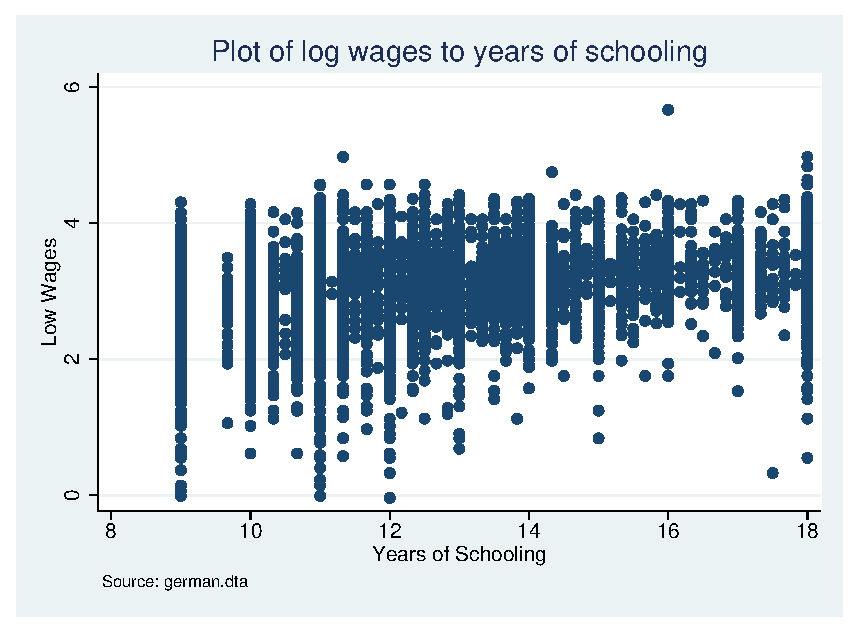
\includegraphics[width=\textwidth]{german-lnw-ed}
  \caption{Scatter plot of log-wages to years of schooling}
   \label{fig:german-lnw-ed}
\end{centering}
\end{figure}

\question{1a4}{Based on the plot, is there any evidence of heteroskedasticity?  }
We notice in the graph in Figure ~\ref{fig:german-lnw-ed} that the variation in the values for each level of years of schooling is not similar. Specifically there seems to be much more variance at ed = 9, ed = 11, ed = 12, and ed = 18. On the other hand, the variation for the period ed=14 to ed=17 seems lower. We may suspect that the level of variance in the error term of our regression may be related to the value of ed. This suggests that heteroskedasticity is a possibility. Had this not been the case, we would have expected to see a similar level of variation in the value of log wages for all values of years of schooling. Clearly that is not the case here. The case for heteroskedasticity is confirmed in the graph in Figure ~\ref{fig:german-res-fit} that plots residuals against the fitted log wages value.

\begin{figure}[h]
\begin{centering}
  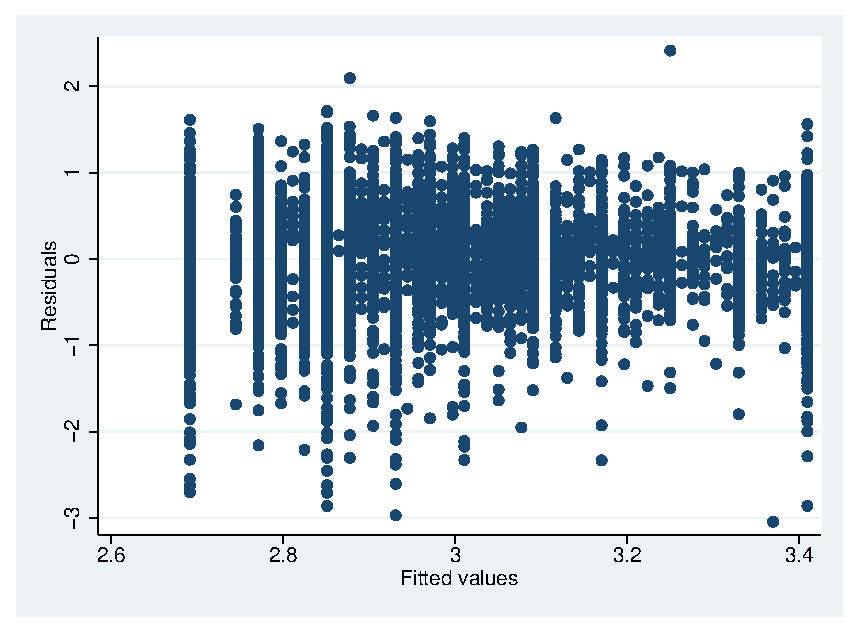
\includegraphics[width=\textwidth]{german-res-fit}
  \caption{Scatter plot of residuals to fitted log wages}
   \label{fig:german-res-fit}
\end{centering}
\end{figure}

\question{1a5}{Now run the multivariate regression of log-wages on a constant, years of schooling, experience, experience-squared, the gender indicator, and the marital status indicators, while adjusting for heteroskedasticity (use "robust" option in STATA).}
\begin{lstlisting}
reg lnw ed exp exp2 female mar, robust
outreg2 using  /Users/aiyenggar/OneDrive/code/articles/adv-eco-hw1-images/02-lnw-ed-all.tex, tex(frag) replace
\end{lstlisting}
\begin{tabular}{lc} \hline
 & (1) \\
VARIABLES & lnw \\ \hline
 &  \\
ed & 0.0809*** \\
 & (0.00121) \\
exp & 0.0309*** \\
 & (0.00111) \\
exp2 & -0.0487*** \\
 & (0.00221) \\
female & -0.213*** \\
 & (0.00604) \\
mar & 0.0398*** \\
 & (0.00633) \\
Constant & 1.626*** \\
 & (0.0196) \\
 &  \\
Observations & 20,042 \\
 R-squared & 0.305 \\ \hline
\multicolumn{2}{c}{ Robust standard errors in parentheses} \\
\multicolumn{2}{c}{ *** p$<$0.01, ** p$<$0.05, * p$<$0.1} \\
\end{tabular}


\question{1a6}{Explain briefly how these estimated standard errors are corrected for heteroskedasticity. }
\begin{figure}[h]
\begin{centering}
  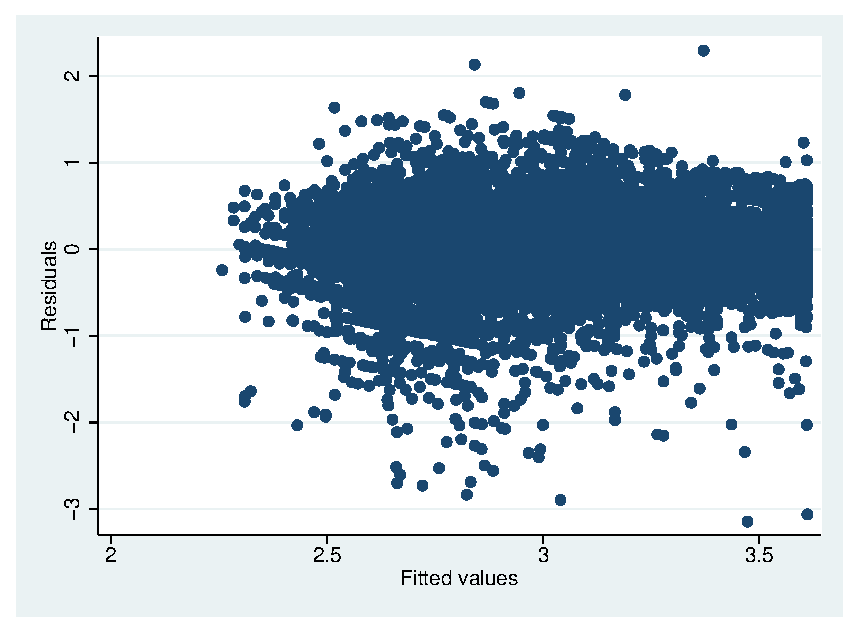
\includegraphics[width=\textwidth]{german-res-fit2}
  \caption{Scatter plot of residuals to fitted log wages in the expanded model}
   \label{fig:german-res-fit2}
\end{centering}
\end{figure}

We learn from theory that the standard errors are biased when heteroskedasticity is present. OLS regression assumes that the error terms are independent and identically distributed (iid), whereas as we noted in Figure ~\ref{fig:german-lnw-ed} and Figure ~\ref{fig:german-res-fit}, that assumption may not quite be true in this case. By relaxing the iid assumption when using the \verb| robust | option, we therefore obtain more trustworthy standard error values (robust standard errors). Additionally, the problem of heteroskedasticity may also be alleviated by a better specification of the model (as seen above), where more variables that influence the outcome of interest are included in the model. In the above, therefore, the estimated standard errors are corrected for heteroskedasticity by a) specifying a fuller model with a greater number of influencing variables, and b) by relaxing the iid assumption in OLS by using the \verb|robust| option in stata. The improved standard errors corrected for heteroskedasticity is visible from Figure ~\ref{fig:german-res-fit2}

Other options to dealing with the problem of heteroskedasticity  is to cluster the data when appropriate (this is adopted in a later question) or to use of weights (the weighted least squares method).

\begin{center}\LARGE{Question 1b}\end{center}
\question{1b}{Now apply the partialling-out method (a.k.a. Frisch-Waugh-Lovell Theorem) to the multivariate regression}

\question{1b1}{run a regression of log-wages on a constant, experience, experience-squared, the gender indicator, and the marital status indicators}
\begin{lstlisting}
reg lnw ed exp exp2 female mar
outreg2 using  /Users/aiyenggar/OneDrive/code/articles/adv-eco-hw1-images/01-par1.tex, tex(frag) replace
\end{lstlisting}
\begin{tabular}{lc} \hline
 & (1) \\
VARIABLES & lnw \\ \hline
 &  \\
exp & 0.0304*** \\
 & (0.00119) \\
exp2 & -0.0576*** \\
 & (0.00234) \\
female & -0.270*** \\
 & (0.00632) \\
mar & 0.0641*** \\
 & (0.00719) \\
Constant & 2.686*** \\
 & (0.0131) \\
 &  \\
Observations & 20,042 \\
 R-squared & 0.133 \\ \hline
\multicolumn{2}{c}{ Standard errors in parentheses} \\
\multicolumn{2}{c}{ *** p$<$0.01, ** p$<$0.05, * p$<$0.1} \\
\end{tabular}


\question{1b2}{save the residuals using STATA command [predict variable name, residual]}
\begin{verbatim}predict r1, resid\end{verbatim}

\question{1b3}{run a regression of years of schooling on a constant, experience, experience-squared, the gender indicator, and the marital status indicators}
\begin{lstlisting}
reg ed exp exp2 female mar
outreg2 using  /Users/aiyenggar/OneDrive/code/articles/adv-eco-hw1-images/01-par2.tex, tex(frag) replace
\end{lstlisting}
\begin{tabular}{lc} \hline
 & (1) \\
VARIABLES & ed \\ \hline
 &  \\
exp & -0.00556 \\
 & (0.00658) \\
exp2 & -0.110*** \\
 & (0.0129) \\
female & -0.700*** \\
 & (0.0348) \\
mar & 0.301*** \\
 & (0.0396) \\
Constant & 13.10*** \\
 & (0.0720) \\
 &  \\
Observations & 20,042 \\
 R-squared & 0.097 \\ \hline
\multicolumn{2}{c}{ Standard errors in parentheses} \\
\multicolumn{2}{c}{ *** p$<$0.01, ** p$<$0.05, * p$<$0.1} \\
\end{tabular}


\question{1b4}{save the residuals; }
\begin{verbatim}predict r2, resid\end{verbatim}


\question{1b5}{regress the residuals from (ii) on the residuals from (iv), while adjusting for heteroskedasticity.}
We perform the regression of r1 on r2 in two ways. First, we do not adjust for heteroskedasticy, and second we use the \verb|robust| option to  control for heteroskedasticity
\begin{lstlisting}
reg r1 r2
outreg2 using  /Users/aiyenggar/OneDrive/code/articles/adv-eco-hw1-images/01-par3.tex, tex(frag) replace
\end{lstlisting}
\begin{tabular}{lc} \hline
 & (1) \\
VARIABLES & r1 \\ \hline
 &  \\
r1 &  \\
 &  \\
 &  \\
r2 & 0.0809*** \\
 & (0.00115) \\
 & 70.48 \\
Constant & 2.82e-10 \\
 & (0.00271) \\
 & 1.04e-07 \\
 &  \\
Observations & 20,042 \\
 R-squared & 0.199 \\ \hline
\multicolumn{2}{c}{ Standard errors in parentheses} \\
\multicolumn{2}{c}{ *** p$<$0.01, ** p$<$0.05, * p$<$0.1} \\
\end{tabular}


\begin{lstlisting}
reg r1 r2, robust
outreg2 using  /Users/aiyenggar/OneDrive/code/articles/adv-eco-hw1-images/01-par3-robust.tex, tex(frag) replace
\end{lstlisting}
\begin{tabular}{lc} \hline
 & (1) \\
VARIABLES & r1 \\ \hline
 &  \\
r1 &  \\
 &  \\
 &  \\
r2 & 0.0809*** \\
 & (0.00121) \\
 & 67.13 \\
Constant & 2.82e-10 \\
 & (0.00271) \\
 & 1.04e-07 \\
 &  \\
Observations & 20,042 \\
 R-squared & 0.199 \\ \hline
\multicolumn{2}{c}{ Robust standard errors in parentheses} \\
\multicolumn{2}{c}{ *** p$<$0.01, ** p$<$0.05, * p$<$0.1} \\
\end{tabular}


\question{1b6}{Compare this regression coefficient to the one (the coefficient on years of schooling) from the multivariate regression in part (a). Are they the same?  What about standard errors and t-statistics?  }
As in the section above, we run the multivariate regression without controlling for heteroskedasticity, and then controlling for heteroskedasticity.

\begin{lstlisting}
reg lnw ed exp exp2 female mar
outreg2 using  /Users/aiyenggar/OneDrive/code/articles/adv-eco-hw1-images/01-par4.tex, tex(frag) replace
\end{lstlisting}
\begin{tabular}{lc} \hline
 & (1) \\
VARIABLES & lnw \\ \hline
 &  \\
lnw &  \\
 &  \\
 &  \\
ed & 0.0809*** \\
 & (0.00115) \\
 & 70.47 \\
exp & 0.0309*** \\
 & (0.00107) \\
 & 28.86 \\
exp2 & -0.0487*** \\
 & (0.00210) \\
 & -23.17 \\
female & -0.213*** \\
 & (0.00572) \\
 & -37.26 \\
mar & 0.0398*** \\
 & (0.00644) \\
 & 6.175 \\
Constant & 1.626*** \\
 & (0.0190) \\
 & 85.35 \\
 &  \\
Observations & 20,042 \\
 R-squared & 0.305 \\ \hline
\multicolumn{2}{c}{ Standard errors in parentheses} \\
\multicolumn{2}{c}{ *** p$<$0.01, ** p$<$0.05, * p$<$0.1} \\
\end{tabular}


The table above lists the results of the multivariate regression not controlling for heteroskedasticity. The coefficient on \verb|ed| is 0.0809, the \verb|standard error| is 0.00115 and the \verb|t-statistic| is 70.47. These values are identical as when \verb|r1| was regressed on \verb|r2| without controlling for heteroskedasticity. This is as expected by the Frisch-Waugh-Lovell theorem, since \verb|reg r1 r2| was nothing but a regression of \verb|lnw| on \verb|ed| after partialling out the effects of \verb|exp|, \verb|exp2|, \verb|female| and \verb|mar|

However, when we compare the results of the regression of \verb|r1| on \verb|r2| with robust standard errors with the multivariate regression without robust standard errors, we note that while the coefficient of \verb|ed| is identical at 0.0809, the \verb|standard error| is higher at 0.00121 and the \verb|t-statistic| is lower at 67.13. By the Frisch-Waugh-Lovell theorem we expect to see the same coefficient values since the use of robust standard errors does not affect the regression coefficients. However, the higher robust standard error is on account of the fact that the variance in the error term was higher when \verb|ed| was farther from its mean value (depicted in the scatter plot in Figure ~\ref{fig:german-res-fit}) normal OLS standard errors are biased down. In the following, we obtain the results of the multivariate regression with robust standard errors.
\begin{lstlisting}
reg lnw ed exp exp2 female mar, robust
outreg2 using  /Users/aiyenggar/OneDrive/code/articles/adv-eco-hw1-images/01-par4-robust.tex, tex(frag) replace
\end{lstlisting}
\input{adv-eco-hw1-images/01-par4-robust.tex}

In the above we now note that the coefficient on \verb|ed|, the \verb|standard error| and the \verb|t-statistic| match with those obtained from the regression of \verb|r1| on \verb|r2| with robust standard errors. (values 0.0809, 0.00121 and 67.13 respectively), thus supporting Frisch-Waugh-Lovell theorem.
\newpage
\begin{center}\LARGE{Question 2a}\end{center}

\question{2a1}{Write down the OLS estimator when the explanatory variable is binary (in a bivariate regression).  }
$lnw = \beta_0 + \beta_1 * computer + \epsilon$

\question{2a2}{Run a regression of log-wages on a constant and the computer indicator.  }
\begin{lstlisting}
reg lnw computer
outreg2 using  /Users/aiyenggar/OneDrive/code/articles/adv-eco-hw1-images/01-lnw-computer.tex, tex(frag) replace
\end{lstlisting}
\input{adv-eco-hw1-images/01-lnw-computer.tex}

\question{2a3}{Do the two sample t-test for the mean difference in log-wages between workers who use computers on the job and non-users (ttest command in STATA). } 
\begin{lstlisting}
ttest lnw, by(computer)
\end{lstlisting}
\begin{figure}[h]
\begin{centering}
  \includegraphics[width=\textwidth]{01-computer-ttest}
  \caption{Two Sample t-test of mean difference in log wages on computer}
   \label{fig:01-computer-ttest}
\end{centering}
\end{figure}

\question{2a4}{Compare the mean difference, standard error and t-statistic to the ones from the bivariate regression.  Are they the same?}
Mean difference is  -.2875494   Standard Error is  .0065046 95\% Confidence Interval is ( -.3002989, -.2747998), t-statistic is  -44.2070 with 20040 degrees of freedom. We reject the null hypothesis that the difference in the means is zero, and conclude that the means values of \verb|lnw| between computer users and non-computer users is different (pvalue is small:  Pr(|T| > |t|) = 0.0000).
In the bivariate regression, the coefficient is  .2875494   Standard Error is .0065046    t-statistic is 44.21   pvalue (P>|t|) is 0.000    and 95\% confidence interval is (.2747998, .3002989). The results are identical except for the sign because computer is a 0/1 variable and the results from the bivariate regression and the two sample t-test on a 0/1 variable are essentially the same.

\begin{center}\LARGE{Question 2b}\end{center}

\question{2b1}{Now regress log-wages on a constant, the computer indicator, years of schooling, experience, experience-squared, the gender indicator, the marital status indicator, female*married, a dummy for part-time worker, living in city, and civil servants, while adjusting for heteroskedasticity.  }
\begin{lstlisting}
reg lnw computer ed exp exp2 female mar femmar part city beamter, robust
outreg2 using  /Users/aiyenggar/OneDrive/code/articles/adv-eco-hw1-images/02b1.tex, tex(frag) replace
\end{lstlisting}
\input{adv-eco-hw1-images/02b1.tex}

\question{2b2}{How does the regression-adjusted estimate of the return to computer use compare to the one from part (a).  }
The coefficient on computer drops from 0.288 to 0.171 though both are highly significant at 0.01 level of significance. This is to be expected since the model is part a was only partially specified, and the effects of other omitted variables would have shown up in the coefficient of computer.

\question{2b3}{What does this imply about the similarity in observables between computer users and non-users? }
The implication is that the log-wages is only partially explained by computer usage, and that factors such as education, experience, married, and civil servant are positively correlated with log wages even after accounting for computer usage. Additionally, we also interpret experience-squared, female and female-married as being negatively correlated with log wages even after accounting for computer usage. Therefore, while computer usage is correlated with higher log-wages, it does not take away the significance of education, experience, gender, marital status and civil servant on the relationship with log-wages.

\begin{center}\LARGE{Question 2c}\end{center}

\question{2c1}{Now compare the mean characteristics (e.g., age, gender, marital status, education (years of schooling), part-time worker, etc.) of computer users to non-users.  Are they statistically different?  }
\begin{lstlisting}
ttest exp, by(computer)
\end{lstlisting}
With a mean difference of 3.467921 and t = 20.1061, we conclude that exp is statistically different between computer users and computer non-users

\begin{lstlisting}
ttest exp2, by(computer)
\end{lstlisting}
With a mean difference of 1.918545 and t = 22.1091, we conclude that exp2 is statistically different between computer users and computer non-users

\begin{lstlisting}
ttest female, by(computer)
\end{lstlisting}
With a mean difference of  .0298382 and t =  4.1543, we conclude that female is statistically different between computer users and computer non-users

\begin{lstlisting}
ttest mar, by(computer)
\end{lstlisting}
With a mean difference of -.0244855  and t =  -3.6891, we conclude that mar is statistically different between computer users and computer non-users

\begin{lstlisting}
ttest ed, by(computer)
\end{lstlisting}
With a mean difference of -1.760921  and t = -50.8628, we conclude that ed is statistically different between computer users and computer non-users

\begin{lstlisting}
ttest part, by(computer)
\end{lstlisting}
With a mean difference of .0629192  and t =  11.5422, we conclude that \verb|part| is statistically different between computer users and computer non-users

\begin{lstlisting}
ttest femmar, by(computer)
\end{lstlisting}
With a mean difference of .0243063 and t =  3.8486, we conclude that \verb|femmar| is statistically different between computer users and computer non-users

\begin{lstlisting}
ttest city, by(computer)
\end{lstlisting}
With a mean difference of -.0397959  and t = -5.7199, we conclude that \verb|city| is statistically different between computer users and computer non-users

\begin{lstlisting}
ttest beamter, by(computer)
\end{lstlisting}
With a mean difference of -.0572623  and t =  -13.1536, we conclude that \verb|beamter| is statistically different between computer users and computer non-users

From the above we note that each of the characteristics tested for are statistically different between computer users and computer non-users.

\question{2c2}{Why might this cast doubt on the causal interpretation of the return to computer use?  }
We noted above that the mean of each of the nine characteristics were significantly different between computer users and computer non-users. This is highly indicative of selection bias, i.e., the sampling is not random but that computer usage ability itself selects for the nine other variables. Therefore, it would be hard to accept any results on such a sample unless the effects of such selection may be controlled for.

\question{2c3}{Can you think of (unobserved) variables that we have not controlled for that may be related to both computer use and log-wages?  }
Education level of parents, and Income level of parents may both be related to whether a person is a computer user or not, as well as to wages. Additionally, the countries where the respondents are resident may also have an impact on the availability of computers and computer education (imagine remote Africa as an example), and therefore of computer skill, as well as to wage levels depending on the status of the country as a mid-income or low-income country.

\question{2c4}{Explain how this could lead to omitted variables bias in the OLS estimate of the return to computer use. } 
Say that computer education was mandatory and enforced in all schools in the United States, and that they were not in India. In this case, the computer skills and the associated wage increase is significantly influenced by  having attended school in a certain country (or alternatively by having had educated parents). If this is accounted for (as it should be), then the coefficient on computer will be that it is more real. However when the country or parents education levels are excluded, OLS will end up overestimating the impact of computer usage on wages, when in fact computer usage was an outcome of superior resources provided due to living in a richer country or having had better educated parents. Omitted variables result in a mis-specification of the model, and are likely to show spurious results.

\begin{center}\LARGE{Question 2d}\end{center}
\question{2d1}{Now add the indicators for calculator, telephone, and pencil use to the regression you ran in part (b).  }
\begin{lstlisting}
reg lnw computer ed exp exp2 female mar femmar part city beamter calc telefon pencil, robust
outreg2 using  /Users/aiyenggar/OneDrive/code/articles/adv-eco-hw1-images/02d1.tex, tex(frag) replace
\end{lstlisting}
\input{adv-eco-hw1-images/02d1.tex}

\question{2d2}{Compare the estimated return to computer use to the one from part (b).  }
The coefficient on the return to computer in this enhanced model is 0.126 as compared with 0.171. Clearly some of the effect seems to have been accounted for by pencil, telefon and calc. However both results are significant at a 0.01 level of significance. The question to be concerned about is if each of calc pencil telefon and computer are themselves an outcome of training, nature of work, country of residence etc, rather than being themselves the source of greater wages.

\question{2d3}{Now run a regression that also controls for the individual\textquotesingle s occupation category as "fixed effects" [areg y x, absorb(occ) robust].  }
\begin{lstlisting}
areg lnw computer ed exp exp2 female mar femmar part city beamter calc telefon pencil, absorb(occ)
outreg2 using  /Users/aiyenggar/OneDrive/code/articles/adv-eco-hw1-images/02d3.tex, tex(frag) replace
\end{lstlisting}
\input{adv-eco-hw1-images/02d3.tex}

\question{2d4}{Interpret the implications of your findings for the role of potential omitted variables bias in the OLS estimate of the effect of computer use on log-wages (see DiNardo and Pischke (1997) for their interpretation).}
When controlled for occupation category,  we see that the ceofficient on \verb|computer| drops from .1257297 to .0694539 though both remain highly significant at 0.01 level of significance and the coefficient on \verb|ed| drops from .0669989  to .040486. This means that different professions have significant differences in wages, and that the occupation itself may convey a significant amount of information about the level of wages. DiNardo, Hallock and Pischke (1997) suggests that the level of unionization may also influence pay. For example therefore, it may be that it is not that the occupation per se determines the level of pay, but some aspect about the occupation (as if it has a unionized workforce) may determine the level of wages. Therefore, we conclude that without strong theoretical backing, it would be inappropriate to conclude much from the estimates of the regression. Omitted variables can distort the picture, and unless we have confidence that the important variables have been captured accurately in the model, we risk spurious results in our interpretation of the regression.

\begin{center}\LARGE{Question 2e}\end{center}

\question{2e1}{Now run the same regression as in part (d), while using the "cluster" option in STATA to correct the estimated standard errors for clustering at the occupation-level [areg y x, absorb(occ) cluster(occ)].  }
\begin{lstlisting}
reg lnw computer ed exp exp2 female mar femmar part city beamter calc telefon pencil, absorb(occ) cluster(occ)
outreg2 using  /Users/aiyenggar/OneDrive/code/articles/adv-eco-hw1-images/02e1.tex, tex(frag) replace
\end{lstlisting}
\begin{tabular}{lc} \hline
 & (1) \\
VARIABLES & lnw \\ \hline
 &  \\
computer & 0.0695*** \\
 & (0.00796) \\
ed & 0.0405*** \\
 & (0.00195) \\
exp & 0.0255*** \\
 & (0.00157) \\
exp2 & -0.0378*** \\
 & (0.00279) \\
female & -0.109*** \\
 & (0.0128) \\
mar & 0.0780*** \\
 & (0.00964) \\
femmar & -0.107*** \\
 & (0.0142) \\
part & 0.0647*** \\
 & (0.0214) \\
city & -0.00820 \\
 & (0.00594) \\
beamter & -0.0492*** \\
 & (0.0119) \\
calc & 0.0224*** \\
 & (0.00779) \\
telefon & 0.0485*** \\
 & (0.0102) \\
pencil & 0.00680 \\
 & (0.00850) \\
Constant & 2.056*** \\
 & (0.0324) \\
 &  \\
Observations & 20,042 \\
 R-squared & 0.445 \\ \hline
\multicolumn{2}{c}{ Robust standard errors in parentheses} \\
\multicolumn{2}{c}{ *** p$<$0.01, ** p$<$0.05, * p$<$0.1} \\
\end{tabular}


\question{2e2}{Explain why the standard error on the estimated return to computer use is higher (and lower t-statistic) than when clustering is not corrected for.}
\verb|cluster| allows for intragroup correlation to be accounted therefore relaxing the assumption that the error terms are all independent of each other. This way, when clustering is used standard errors are expected to be calculated based on variation within the cluster rather than across the entire data sample. Clearly therefore clustering should lower the standard errors of the estimates as compared to not clustering.
\newpage
\begin{center}\LARGE{Question 3a}\end{center}

\question{3a1}{ Use experimental data [experimt==1].  Test the mean differences in characteristics (e.g., age, race, ethnicity, marital status, and years of schooling) between treatment and control group.  }
\begin{lstlisting}
use NSW_lalonde, clear
keep if experimt==1

ttest age, by(treat)
\end{lstlisting}
With a mean difference of -.1792038  and t =   -0.3574, we conclude that \verb|age| is NOT statistically different by treatment

\begin{lstlisting}
ttest educ, by(treat)
\end{lstlisting}
With a mean difference of -.1922361   and t =   -1.4922, we conclude that \verb|educ| is NOT statistically different by treatment

\begin{lstlisting}
ttest black, by(treat)
\end{lstlisting}
With a mean difference of -.0013468    and t =   -0.0445, we conclude that \verb|black| is NOT statistically different by treatment

\begin{lstlisting}
ttest hispanic, by(treat)
\end{lstlisting}
With a mean difference of  .0186651    and t =  0.8034, we conclude that \verb|hispanic| is NOT statistically different by treatment

\begin{lstlisting}
ttest married, by(treat)
\end{lstlisting}
With a mean difference of  -.0107031 and t = -0.3836, we conclude that \verb|married| is NOT statistically different by treatment

\begin{lstlisting}
ttest nodegree, by(treat)
\end{lstlisting}
With a mean difference of  .0834779 and t =  2.6730, we conclude that \verb|nodegree| \textbf{is}  statistically different by treatment


\question{3a2}{ What does the result of this test imply about the identification of the causal effect of the NSW program?  }
We find that \verb|nodegree| is statistically different by \verb|treat|. This implies that there may be a selection bias in the selection of the treatment group dependent on whether respondents had a high school degree or not. However on all the other parameters on age, education, ethnicity and marriage there is no statistical difference between the treatment group and the control group. In interpreting any results therefore, the effect of high school degree will have to be additionally controlled for.

\question{3a3}{Estimate the average causal effect of the NSW program on earnings (re78) using a regression: i) without control variables; and ii) with control variables (age, educ, black, hispanic, married, nodegree, re75).  }
\begin{lstlisting}
reg re78 treat
outreg2 using  /Users/aiyenggar/OneDrive/code/articles/adv-eco-hw1-images/03a3-base.tex, tex(frag) replace
reg re78 treat age educ black hispanic married nodegree re75
outreg2 using  /Users/aiyenggar/OneDrive/code/articles/adv-eco-hw1-images/03a3-control.tex, tex(frag) replace
\end{lstlisting}
\begin{tabular}{lc} \hline
 & (1) \\
VARIABLES & re78 \\ \hline
 &  \\
treat & 886.3* \\
 & (472.1) \\
Constant & 5,090*** \\
 & (302.8) \\
 &  \\
Observations & 722 \\
 R-squared & 0.005 \\ \hline
\multicolumn{2}{c}{ Standard errors in parentheses} \\
\multicolumn{2}{c}{ *** p$<$0.01, ** p$<$0.05, * p$<$0.1} \\
\end{tabular}

\begin{tabular}{lc} \hline
 & (1) \\
VARIABLES & re78 \\ \hline
 &  \\
treat & 806.5* \\
 & (467.9) \\
age & 17.39 \\
 & (36.19) \\
educ & 175.3 \\
 & (179.6) \\
black & -1,446* \\
 & (801.5) \\
hispanic & 98.42 \\
 & (1,046) \\
married & 71.86 \\
 & (652.3) \\
nodegree & -470.4 \\
 & (742.9) \\
re75 & 0.170*** \\
 & (0.0467) \\
Constant & 3,880 \\
 & (2,604) \\
 &  \\
Observations & 722 \\
 R-squared & 0.043 \\ \hline
\multicolumn{2}{c}{ Standard errors in parentheses} \\
\multicolumn{2}{c}{ *** p$<$0.01, ** p$<$0.05, * p$<$0.1} \\
\end{tabular}


\question{3a4}{Interpret the results.  Are these two estimates (with and without controls) statistically same?  Why would this be the case?}
In both the regressions above, we note that the coefficient of \verb|treat| is positive and significant at the 0.1 level of significance. Therefore the two estimates are indeed statistically the same, thought he coefficient does drop from 886.3 to 806.5. This is so because, with the exception of \verb|nodegree|, we found that the treatment group and the control group were similar on all other variables. This demonstrates that, with the single exception, the samples were randomized, and therefore the impact of controlling on those variables is limited. We also note that \verb|black| is negatively and significant at 0.10 level of significance correlated with \verb|re78|. I also regressed \verb|re78| on \verb|treat| and \verb|nodegree| and found that the coefficient on \verb|nodegree| is significant and negative at a 0.05 level of significance, white \verb|treat| continues to remain significant at a 0.10 level of significance.

\begin{center}\LARGE{Question 3b}\end{center}

\question{3b1}{ Now use the non-experimental control group from the CPS data, along with the experimental treatment group [(experimt==0 \& treat==0)|treat==1].  }
\begin{lstlisting}
use NSW_lalonde, clear
keep if (experimt==0 & treat==0)|treat==1
\end{lstlisting}

\question{3b2}{As you did in part (a), test the mean differences in characteristics between treatment and control group.  }
\begin{lstlisting}
ttest age, by(treat)
\end{lstlisting}
With a mean difference of  8.598975  and t =   13.3712, we conclude that \verb|age| is  statistically different by treatment

\begin{lstlisting}
ttest educ, by(treat)
\end{lstlisting}
With a mean difference of  1.647042  and t =   9.8504, we conclude that \verb|educ| is statistically different by treatment

\begin{lstlisting}
ttest black, by(treat)
\end{lstlisting}
With a mean difference of   -.72781  and t =  -47.0413, we conclude that \verb|black| is  statistically different by treatment

\begin{lstlisting}
ttest hispanic, by(treat) 
\end{lstlisting}
With a mean difference of -.0222401   and t =    -1.4651, we conclude that \verb|hispanic| is NOT statistically different by treatment

\begin{lstlisting}
ttest married, by(treat)
\end{lstlisting}
With a mean difference of  .5433807  and t = 20.5430, we conclude that \verb|married| is  statistically different by treatment

\begin{lstlisting}
ttest nodegree, by(treat)
\end{lstlisting}
With a mean difference of  -.4348043  and t =   -16.2744, we conclude that \verb|nodegree| is  statistically different by treatment

\question{3b3}{ Interpret the results.  }
In the above, we find that except for \verb|hispanic|, all other measures are statistically different between treatment group and control group. This implies that while we make any interpretations, adequate controls need to be applied for where there has been a non-random selection on certain variables.
\question{3b4}{ Again, as you did in part (a), run a regression of earnings (re78) on treatment dummy (treat): i) without control variables; and ii) with control variables.  Interpret the results.  }
\begin{lstlisting}
reg re78 treat
outreg2 using  /Users/aiyenggar/OneDrive/code/articles/adv-eco-hw1-images/03b4-base.tex, tex(frag) replace
reg re78 treat age educ black hispanic married nodegree re75
outreg2 using  /Users/aiyenggar/OneDrive/code/articles/adv-eco-hw1-images/03b4-control.tex, tex(frag) replace
\end{lstlisting}
\begin{tabular}{lc} \hline
 & (1) \\
VARIABLES & re78 \\ \hline
 &  \\
treat & -8,870*** \\
 & (562.5) \\
Constant & 14,847*** \\
 & (75.95) \\
 &  \\
Observations & 16,289 \\
 R-squared & 0.015 \\ \hline
\multicolumn{2}{c}{ Standard errors in parentheses} \\
\multicolumn{2}{c}{ *** p$<$0.01, ** p$<$0.05, * p$<$0.1} \\
\end{tabular}

\begin{tabular}{lc} \hline
 & (1) \\
VARIABLES & re78 \\ \hline
 &  \\
treat & -992.9** \\
 & (451.6) \\
age & -76.41*** \\
 & (5.883) \\
educ & 140.0*** \\
 & (29.03) \\
black & -849.5*** \\
 & (214.6) \\
hispanic & -387.9* \\
 & (221.1) \\
married & 437.3*** \\
 & (143.8) \\
nodegree & 152.8 \\
 & (179.7) \\
re75 & 0.709*** \\
 & (0.00688) \\
Constant & 5,755*** \\
 & (452.1) \\
 &  \\
Observations & 16,289 \\
 R-squared & 0.458 \\ \hline
\multicolumn{2}{c}{ Standard errors in parentheses} \\
\multicolumn{2}{c}{ *** p$<$0.01, ** p$<$0.05, * p$<$0.1} \\
\end{tabular}


For the non-experimental group, we note that the coefficient of \verb|treat| is negative and significant at 0.01 level of significance without controls, and negative and significant at 0.05 level of significance with controls. As expected, we find that \verb|hispanic| is less significant than other controls, though it is itself negative and significant at the 0.10 level of significance. We note that \verb|educ|, \verb|married|, and \verb|re75| have positive coefficients, but that \verb|age|, \verb|black| and \verb|treatment| have negative coefficients.
\question{3b5}{ How do these results compare to the causal estimates using experimental data in part (a)? }
The experimental and non-experimental data throw up very different results. First, we must note that the sample characteristics are significantly different between the two as evidenced by the two-sample mean t-tests performed. While on the experimental group, treatment was found to have a positive and significant (at 0.10 level of significance) effect on \verb|re78|, the effect is negative and significant (at 0.01 level of significance) for the non-experimental data. Since this is the case despite controlling for education, ethnicity, marriage status and 1975 earnings, we must call into question if the model has been appropriately specified. What is consistent between the two is that \verb|re75| is positively correlated with \verb|re78|, and that \verb|black| is negatively correlated with \verb|re78|. Both these results seem consistent with prior findings. However the effect of treatment throws up the biggest challenge. We need to consider possible questions of measurement error, or of a modeling error due to omitted variables. Could there be regional variations or is there possibly a clustering of the data collected on any particular variable that has not been captured in the model? Are there any idiosyncratic aspects about either the randomization of the CPS data? Clearly our two-sample t-test results demonstrate that the CPS data characteristics are different from those of the experimental data. We need to find those differences and account for that in the model. 


\bibliography{/Users/aiyenggar/OneDrive/code/bibliography/ae,/Users/aiyenggar/OneDrive/code/bibliography/fj,/Users/aiyenggar/OneDrive/code/bibliography/ko,/Users/aiyenggar/OneDrive/code/bibliography/pt,/Users/aiyenggar/OneDrive/code/bibliography/uz} 
\bibliographystyle{apalike}


\end{document}
